\clearpage
\setcounter{page}{1}
\maketitlesupplementary


% \section{Rationale}
% \label{sec:rationale}
% % 
% Having the supplementary compiled together with the main paper means that:
% % 
% \begin{itemize}
% \item The supplementary can back-reference sections of the main paper, for example, we can refer to \cref{sec:intro};
% \item The main paper can forward reference sub-sections within the supplementary explicitly (e.g. referring to a particular experiment); 
% \item When submitted to arXiv, the supplementary will already included at the end of the paper.
% \end{itemize}
% % 
% To split the supplementary pages from the main paper, you can use \href{https://support.apple.com/en-ca/guide/preview/prvw11793/mac#:~:text=Delete%20a%20page%20from%20a,or%20choose%20Edit%20%3E%20Delete).}{Preview (on macOS)}, \href{https://www.adobe.com/acrobat/how-to/delete-pages-from-pdf.html#:~:text=Choose%20%E2%80%9CTools%E2%80%9D%20%3E%20%E2%80%9COrganize,or%20pages%20from%20the%20file.}{Adobe Acrobat} (on all OSs), as well as \href{https://superuser.com/questions/517986/is-it-possible-to-delete-some-pages-of-a-pdf-document}{command line tools}.

\section{Robustness of rendering-based methods.}
\label{sup:render_views}
\begin{figure}[htbp]
  \centering
  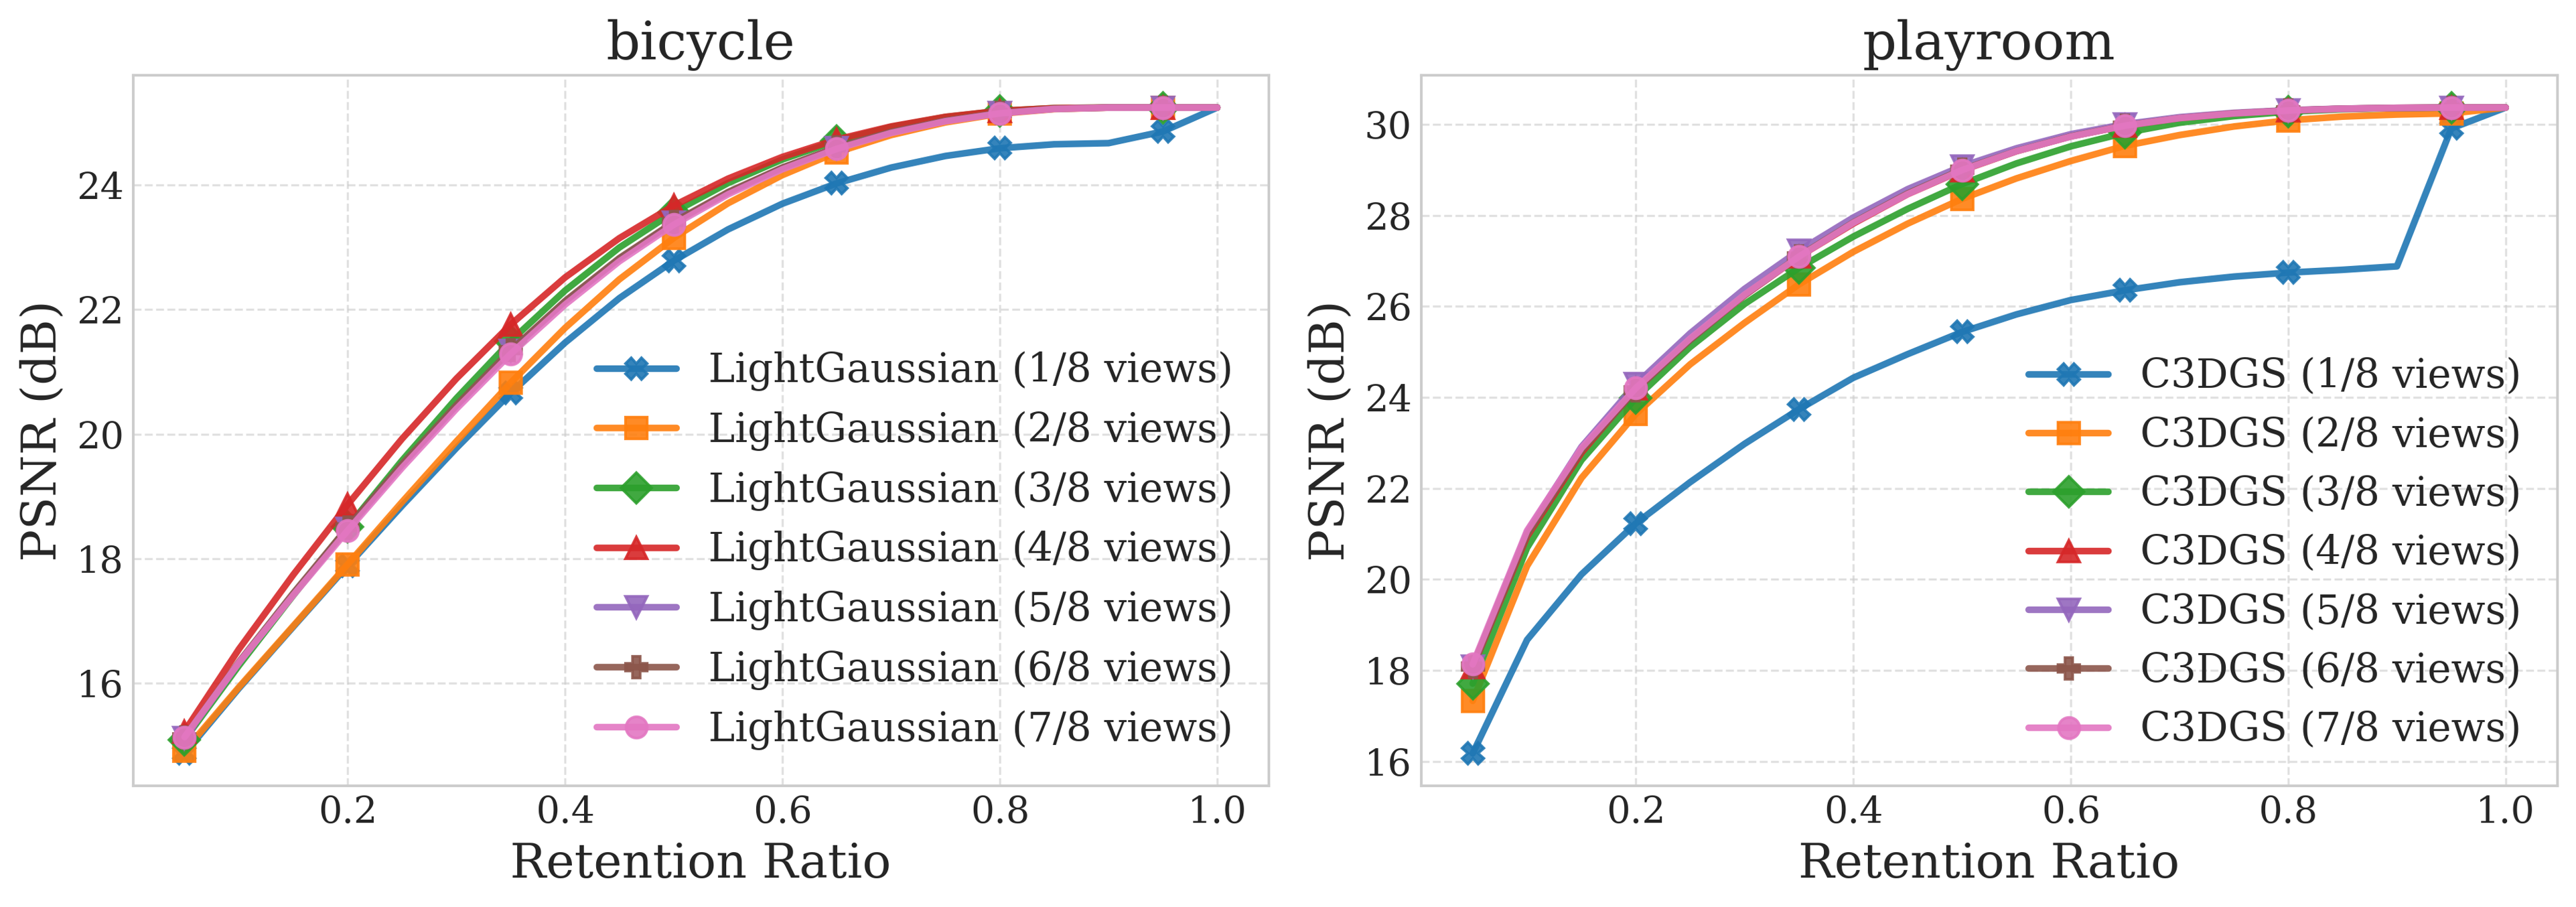
\includegraphics[width=\linewidth]{sec/imgs_sup/viewnumber.png}
  \caption{
  Robustness of rendering-based importance estimation to the number of training views used.
  Left: LightGaussian on the \textit{bicycle} scene from Mip-NeRF360-Outdoor. 
  Right: C3DGS on the \textit{playroom} scene from Deep Blending.
  Each curve corresponds to a different subset of views ($1/8$–$7/8$) used for score computation.
  }
  \label{fig:ablation_viewnum}
\end{figure}

As discussed in Section~\ref{sec:exp_imp}, rendering-based baselines estimate importance by projecting Gaussians from all available training views (i.e., $7/8$ of the total views). 
To analyze their sensitivity to the number of views, we uniformly subsample $1/8$, $2/8$, $\dots$, $7/8$ of the training views to recompute importance scores and evaluate post-hoc pruning results.
As shown in Fig.~\ref{fig:ablation_viewnum}, rendering-based methods exhibit notable instability when the number or distribution of input views changes. 
For instance, LightGaussian’s pruning quality on the \textit{bicycle} scene fluctuates by up to 1.5~dB PSNR across different view counts, while C3DGS on \textit{playroom} suffers a 4~dB drop when using only $1/8$ of the views and still varies by about 1~dB across the remaining subsets. 
Besides, using more views does not always yield better scores: LightGaussian achieves its best performance with $4/8$ views, and C3DGS peaks at $5/8$.
These results suggest that rendering-based importance estimation is highly dependent on the number and spatial distribution of selected views, 
whereas our RAP, relying solely on point-level features without rendering, is inherently view-agnostic and thus more robust.

\section{Post-hoc Pruning: Additional Results}
\label{sup:post_hoc}

\begin{figure*}[htpb]
  \centering
  \begin{minipage}{0.48\linewidth}
    \centering
    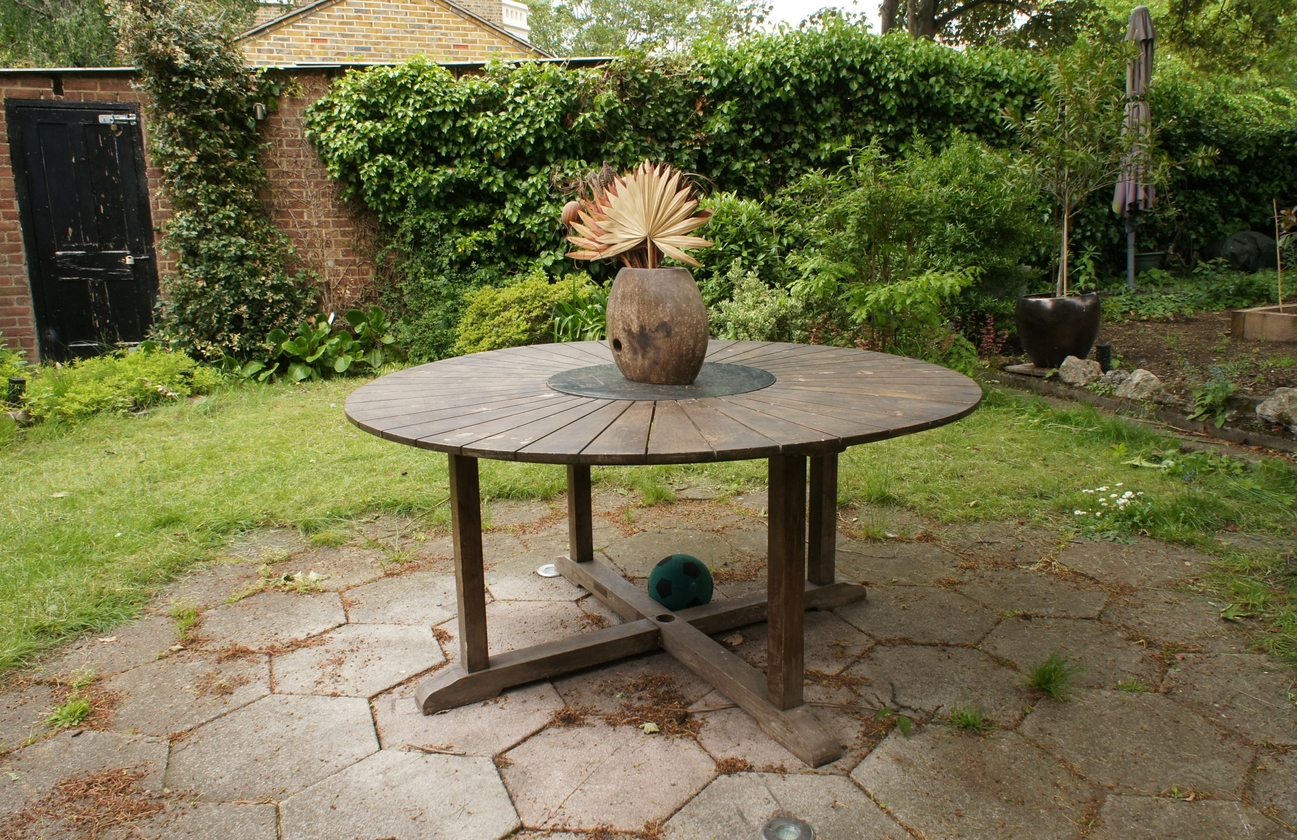
\includegraphics[width=\linewidth]{sec/imgs_sup/garden.png}
    \vspace{2pt}
    \small (a) Original scene
  \end{minipage}
  \hfill
  \begin{minipage}{0.48\linewidth}
    \centering
    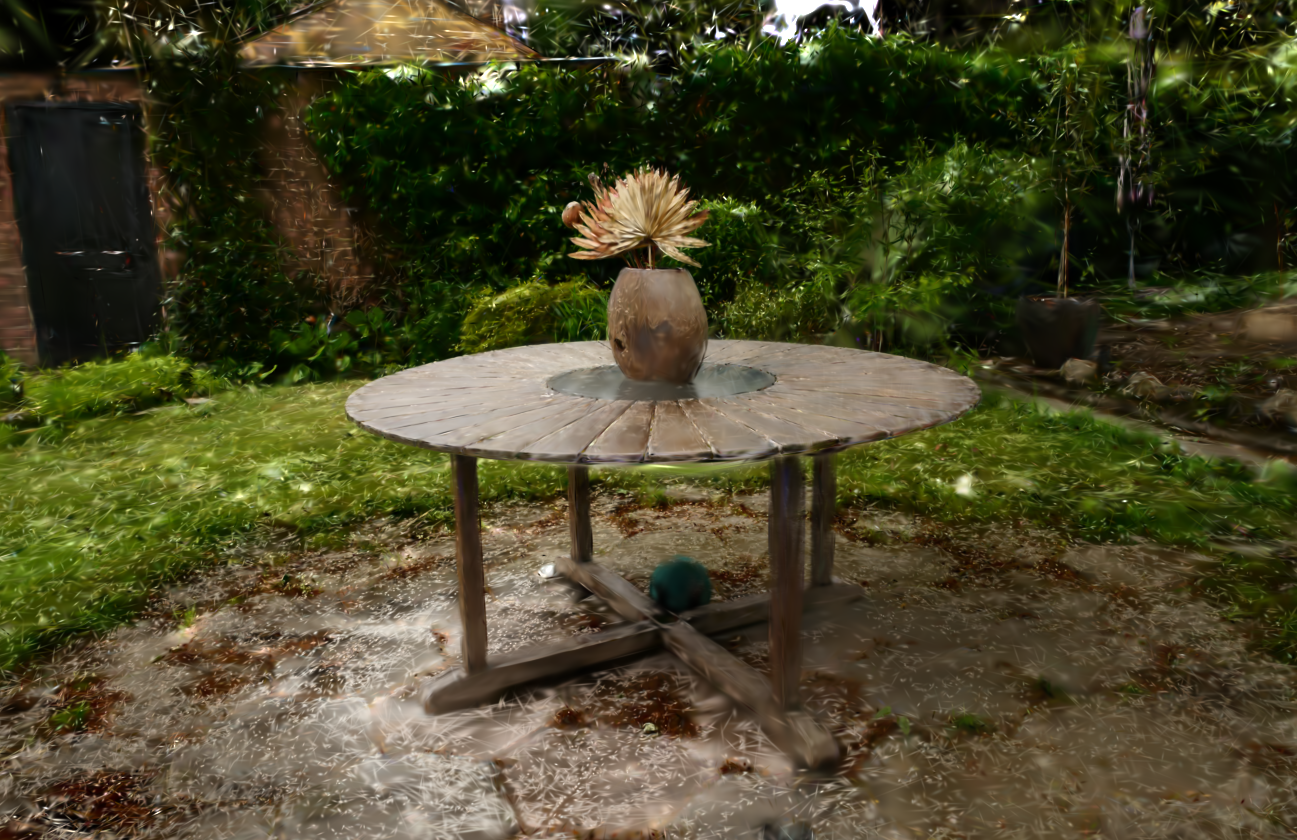
\includegraphics[width=\linewidth]{sec/imgs_sup/garden_rap.png}
    \vspace{2pt}
    \small (b) RAP (ours, 5\% retained)
  \end{minipage}
  \vspace{4pt}
  \begin{minipage}{0.48\linewidth}
    \centering
    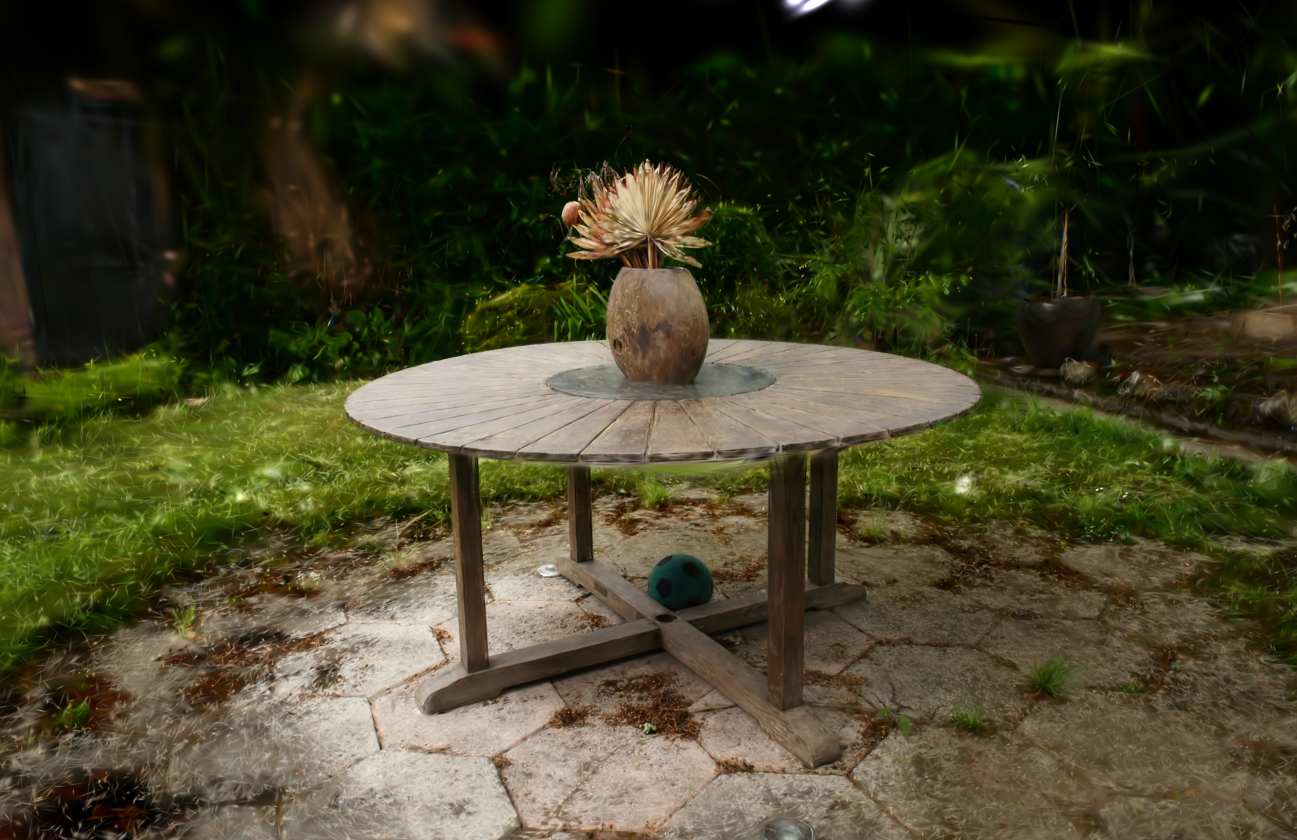
\includegraphics[width=\linewidth]{sec/imgs_sup/garden_eagles.png}
    \vspace{2pt}
    \small (c) EAGLES (visibility-based, 5\% retained)
  \end{minipage}
  \hfill
  \begin{minipage}{0.48\linewidth}
    \centering
    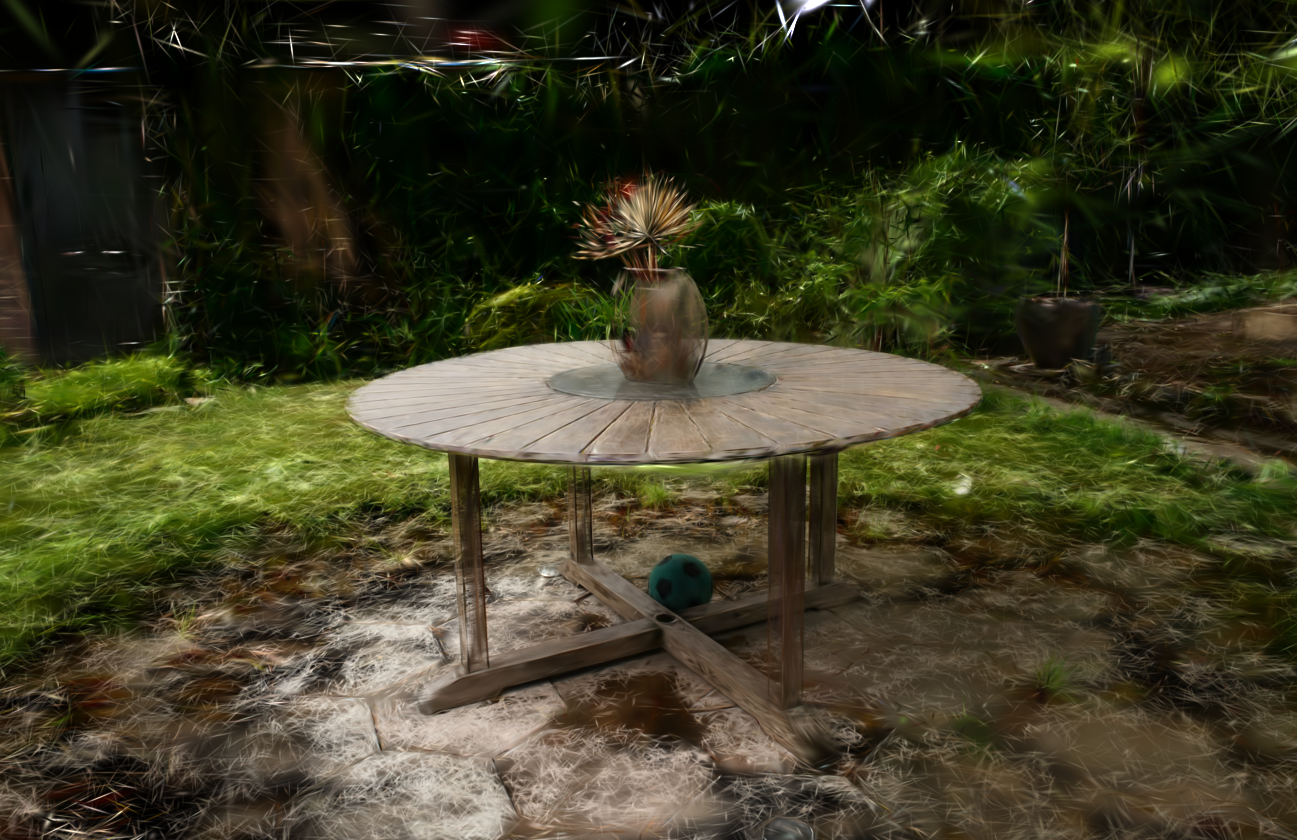
\includegraphics[width=\linewidth]{sec/imgs_sup/garden_c3dgs.png}
    \vspace{2pt}
    \small (d) C3DGS (gradient-based, 5\% retained)
  \end{minipage}
  \vspace{4pt}
  \caption{
    Pruning behavior of different importance estimators at 5\% retention. 
    EAGLES favors central regions, C3DGS keeps edges, while RAP produces a more uniform, structure-preserving subset.
  }
  \label{fig:exp_garden_vis}
\end{figure*}


Per-scene results are shown in Fig.~\ref{fig:sup_2_metrics}, RAP consistently achieves the highest PSNR on nearly all scenes, with the only exceptions being \textit{bicycle} and \textit{stump} from the Mip-NeRF360 Outdoor dataset, where EAGLES is approximately 0.3\,dB better around the 60\% pruning ratio. 
Visibility-based approaches such as LightGaussian, MesonGS, and EAGLES tend to perform slightly worse than RAP (typically within 0.3\,dB). 
Although these methods differ in their use of opacity, blending opacity, or volume weighting, their overall behavior is largely comparable. Each achieves slightly better results on certain scenes and slightly worse on others, but none exhibits a consistent or systematic advantage across datasets.

In contrast, gradient-based methods (C3DGS, PUP-3DGS) are far less stable. 
They show substantial degradation on several scenes---\textit{kitchen}, \textit{playroom}, \textit{truck}, and \textit{train}---where their PSNR drops by 2--3\,dB relative to RAP. 
At certain pruning ratios, their performance even falls below the naive opacity baseline (e.g., C3DGS on \textit{playroom}, PUP-3DGS on \textit{truck}).

For SSIM and LPIPS, RAP typically ranks second or third on most Mip-NeRF360 scenes, with EAGLES often obtaining the best perceptual scores. 
To better understand these differences, we visualize the retained primitives on the \textit{garden} scene in Fig.~\ref{fig:exp_garden_vis}. 
The comparison reveals distinct selection biases across methods:
\begin{itemize}
    \item \textbf{Visibility-based methods (e.g., EAGLES).}
    These methods strongly favor primitives near the scene center. 
    This arises because: 
    (1) training views surround the central object, causing central primitives to accumulate many projected contributions while background primitives receive far fewer; and 
    (2) projected area decreases with depth, causing distant primitives to appear smaller and thus receive lower scores. 
    Consequently, foreground structures are well preserved, but background regions are severely underrepresented.
    \item \textbf{Gradient-based methods (e.g., C3DGS).}
    These approaches mainly retain high-frequency edges, while smooth surfaces lose most of their support. 
    Under heavy pruning, this leads to incomplete geometry and strong artifacts.
    \item \textbf{RAP (ours).}
    RAP produces a more uniform selection across the entire scene, preserving both foreground and background content. 
    This explains why RAP achieves the strongest PSNR across datasets---PSNR benefits from globally consistent coverage---whereas SSIM and LPIPS, which emphasize structural similarity, may sometimes favor visibility-based techniques.
\end{itemize}

% \section{In-Loop Pruning: Additional Results}
% \label{sup:prune_in_loop}
% \begin{figure*}[htbp]
%     \centering

%     \begin{subfigure}{0.95\linewidth}
%         \centering
%         \includegraphics[width=\linewidth]{sec/imgs_sup/playroom_00018_diff_original.png}
%         \caption{Original 3DGS: input view, rendering, and error map.}
%     \end{subfigure}

%     \vspace{0.6em}

%     \begin{subfigure}{0.95\linewidth}
%         \centering
%         \includegraphics[width=\linewidth]{sec/imgs_sup/playroom_00018_diff_RAP.png}
%         \caption{3DGS trained with RAP pruning: input view, rendering, and error map.}
%     \end{subfigure}

%     \caption{
%     Reconstruction comparison before and after integrating RAP into the 3DGS training loop.
%     }
%     \label{fig:playroom_diff}
% \end{figure*}
% As we stated in Sec.~\ref{sec:exp2_rec_pruning}, 
% \section{MPEG GSC: Additional Experimental Results}

\section{Loss Function Analysis and Score Distribution Visualization}
\label{sup:loss}

\begin{figure}[t]
    \centering

    \begin{subfigure}{0.48\linewidth}
        \centering
        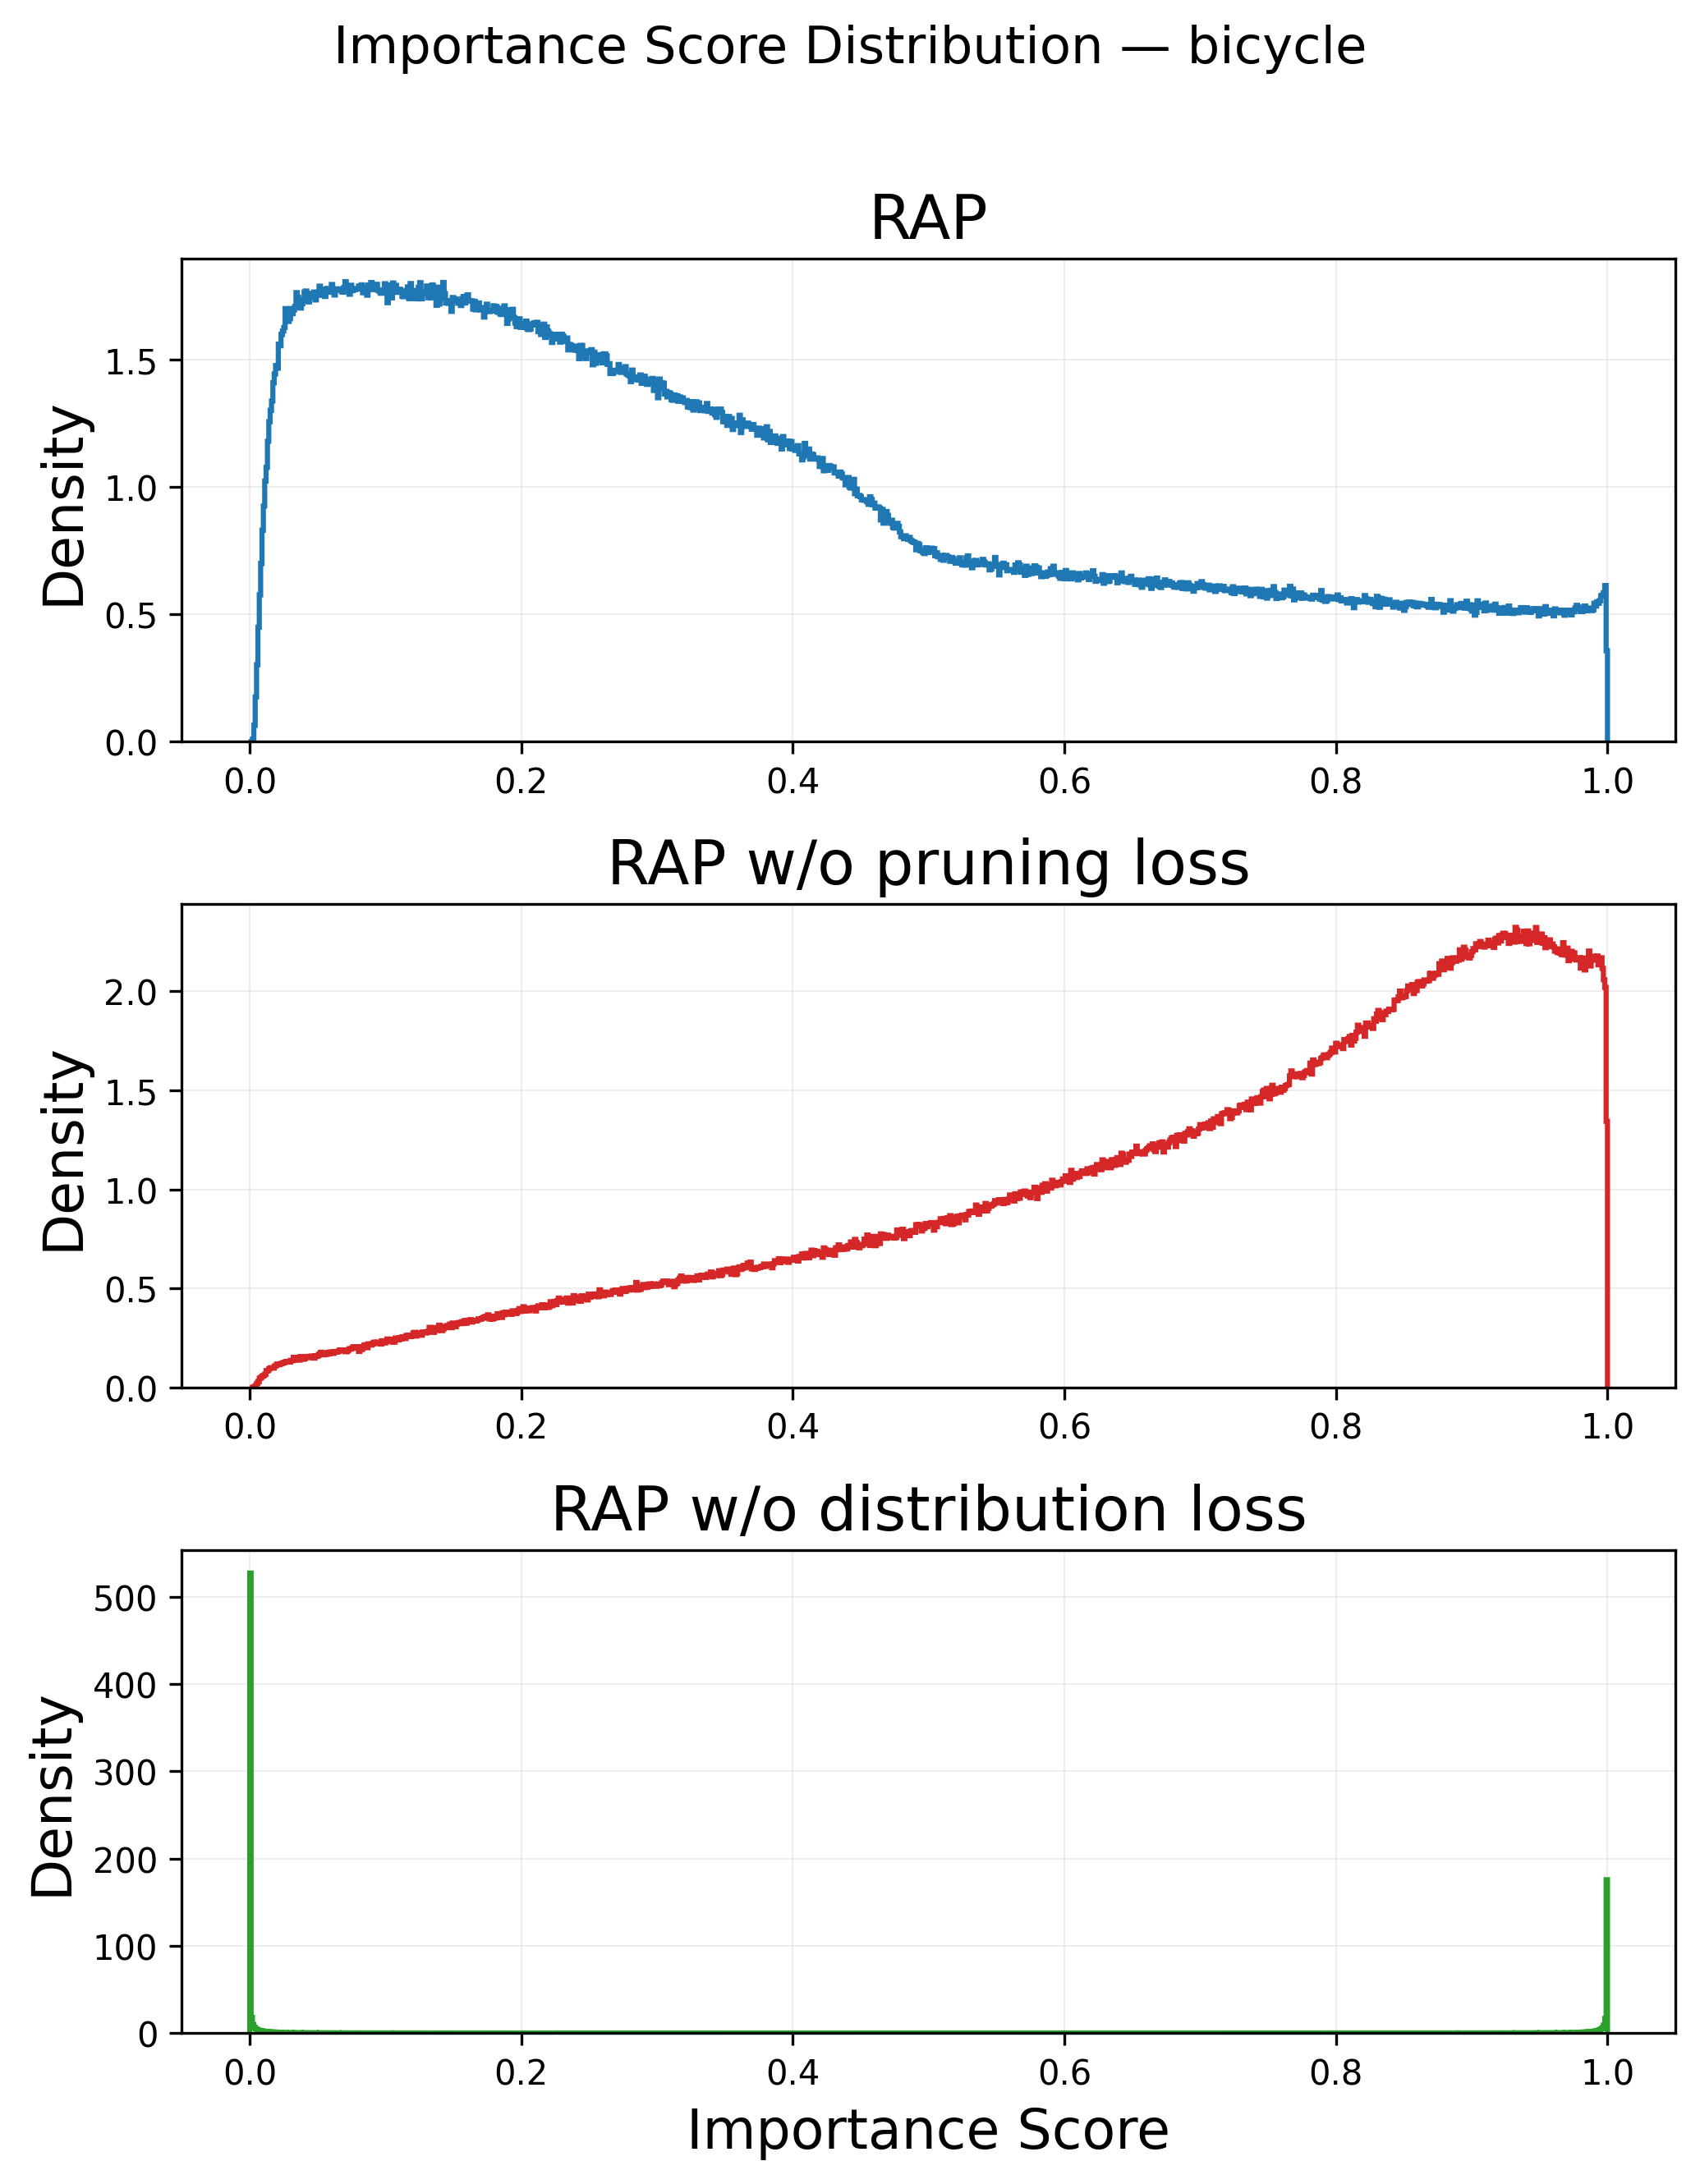
\includegraphics[width=\linewidth]{sec/imgs_sup/bicycle_score_distribution.png}
    \end{subfigure}
    \hfill
    \begin{subfigure}{0.48\linewidth}
        \centering
        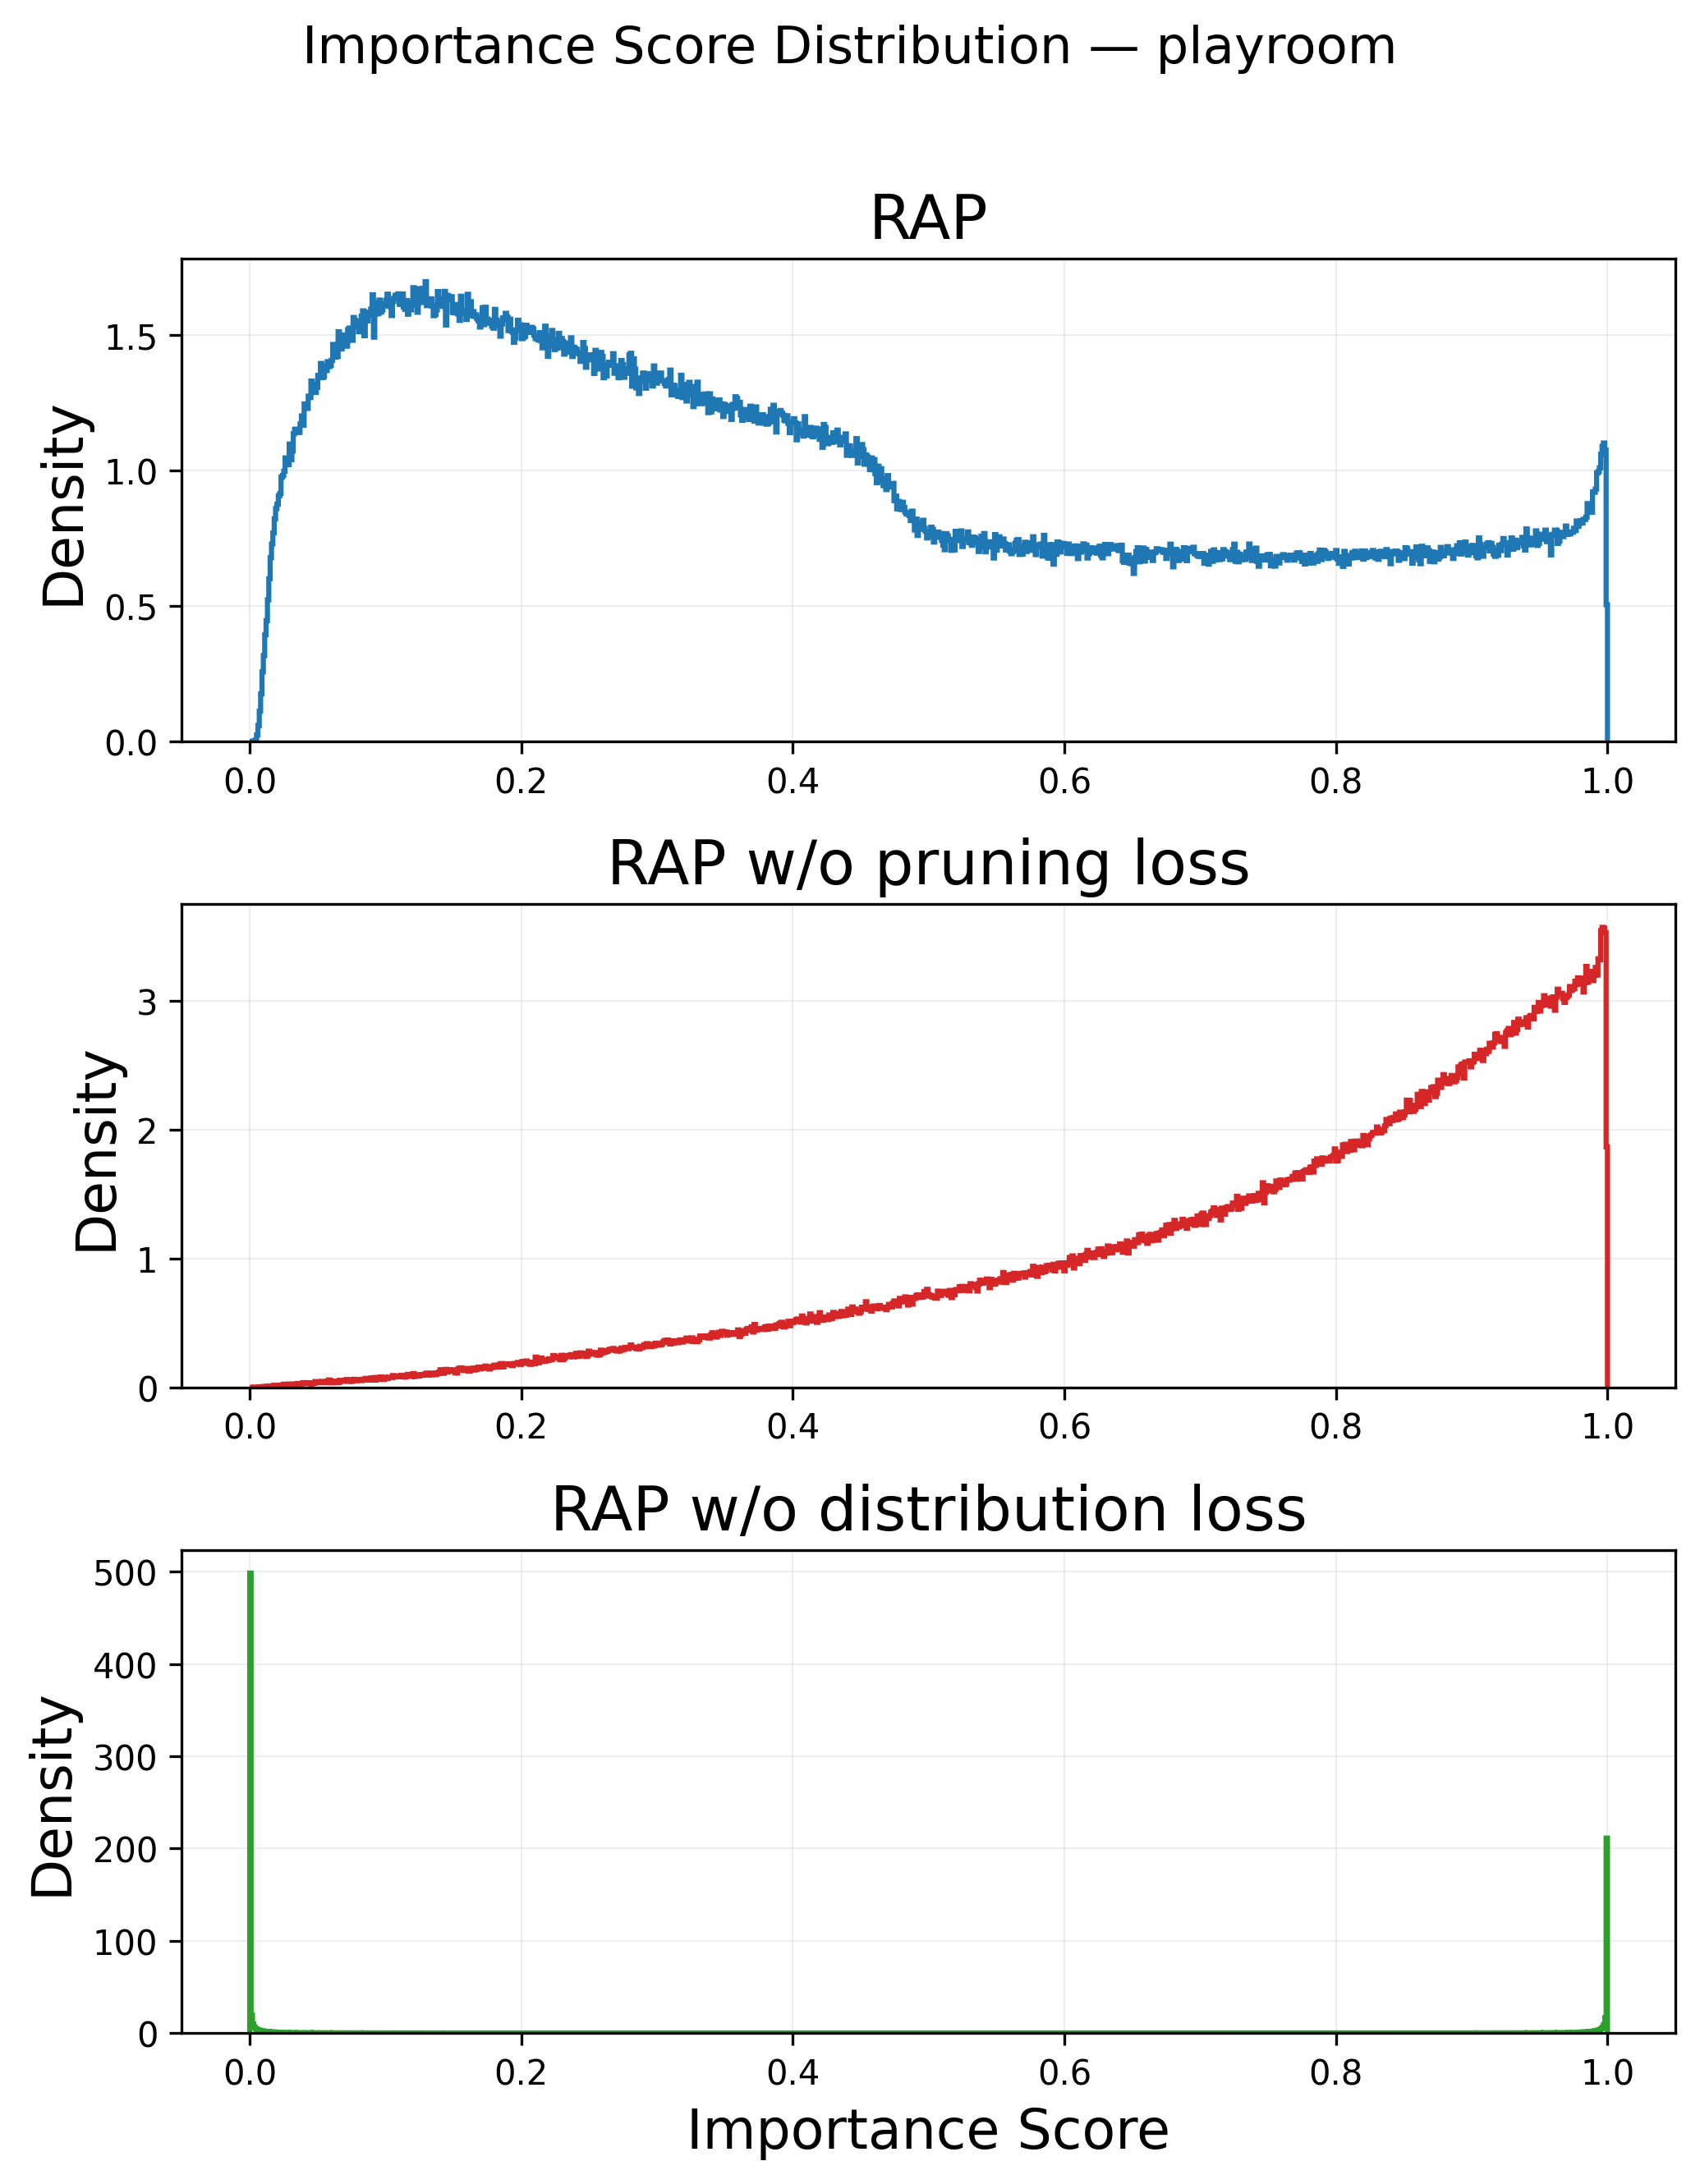
\includegraphics[width=\linewidth]{sec/imgs_sup/playroom_score_distribution.png}
    \end{subfigure}

    \caption{
    Predicted score distributions for RAP, RAP without pruning-aware loss, 
    and RAP without distribution loss.
    }
    \label{fig:sup_score_distribution}
\end{figure}

To better understand how the pruning-aware loss and the distribution regularization shape the predicted scores, Fig.~\ref{fig:sup_score_distribution} visualizes the score distributions produced by RAP and its ablated variants.
Without the pruning-aware loss, the network tends to assign overly large scores to most primitives, making it difficult to identify truly important points.
In contrast, removing the distribution loss causes the scores to collapse toward near-binary values around 0 and 1, which prevents setting flexible pruning thresholds and makes fine-grained importance discrimination unreliable.
The full RAP model produces a smooth and well-spread distribution—dominated by low scores but with clear separation among mid- and high-importance primitives—enabling stable and accurate pruning across a wide range of ratios.



\begin{figure*}[htbp]
  \centering
  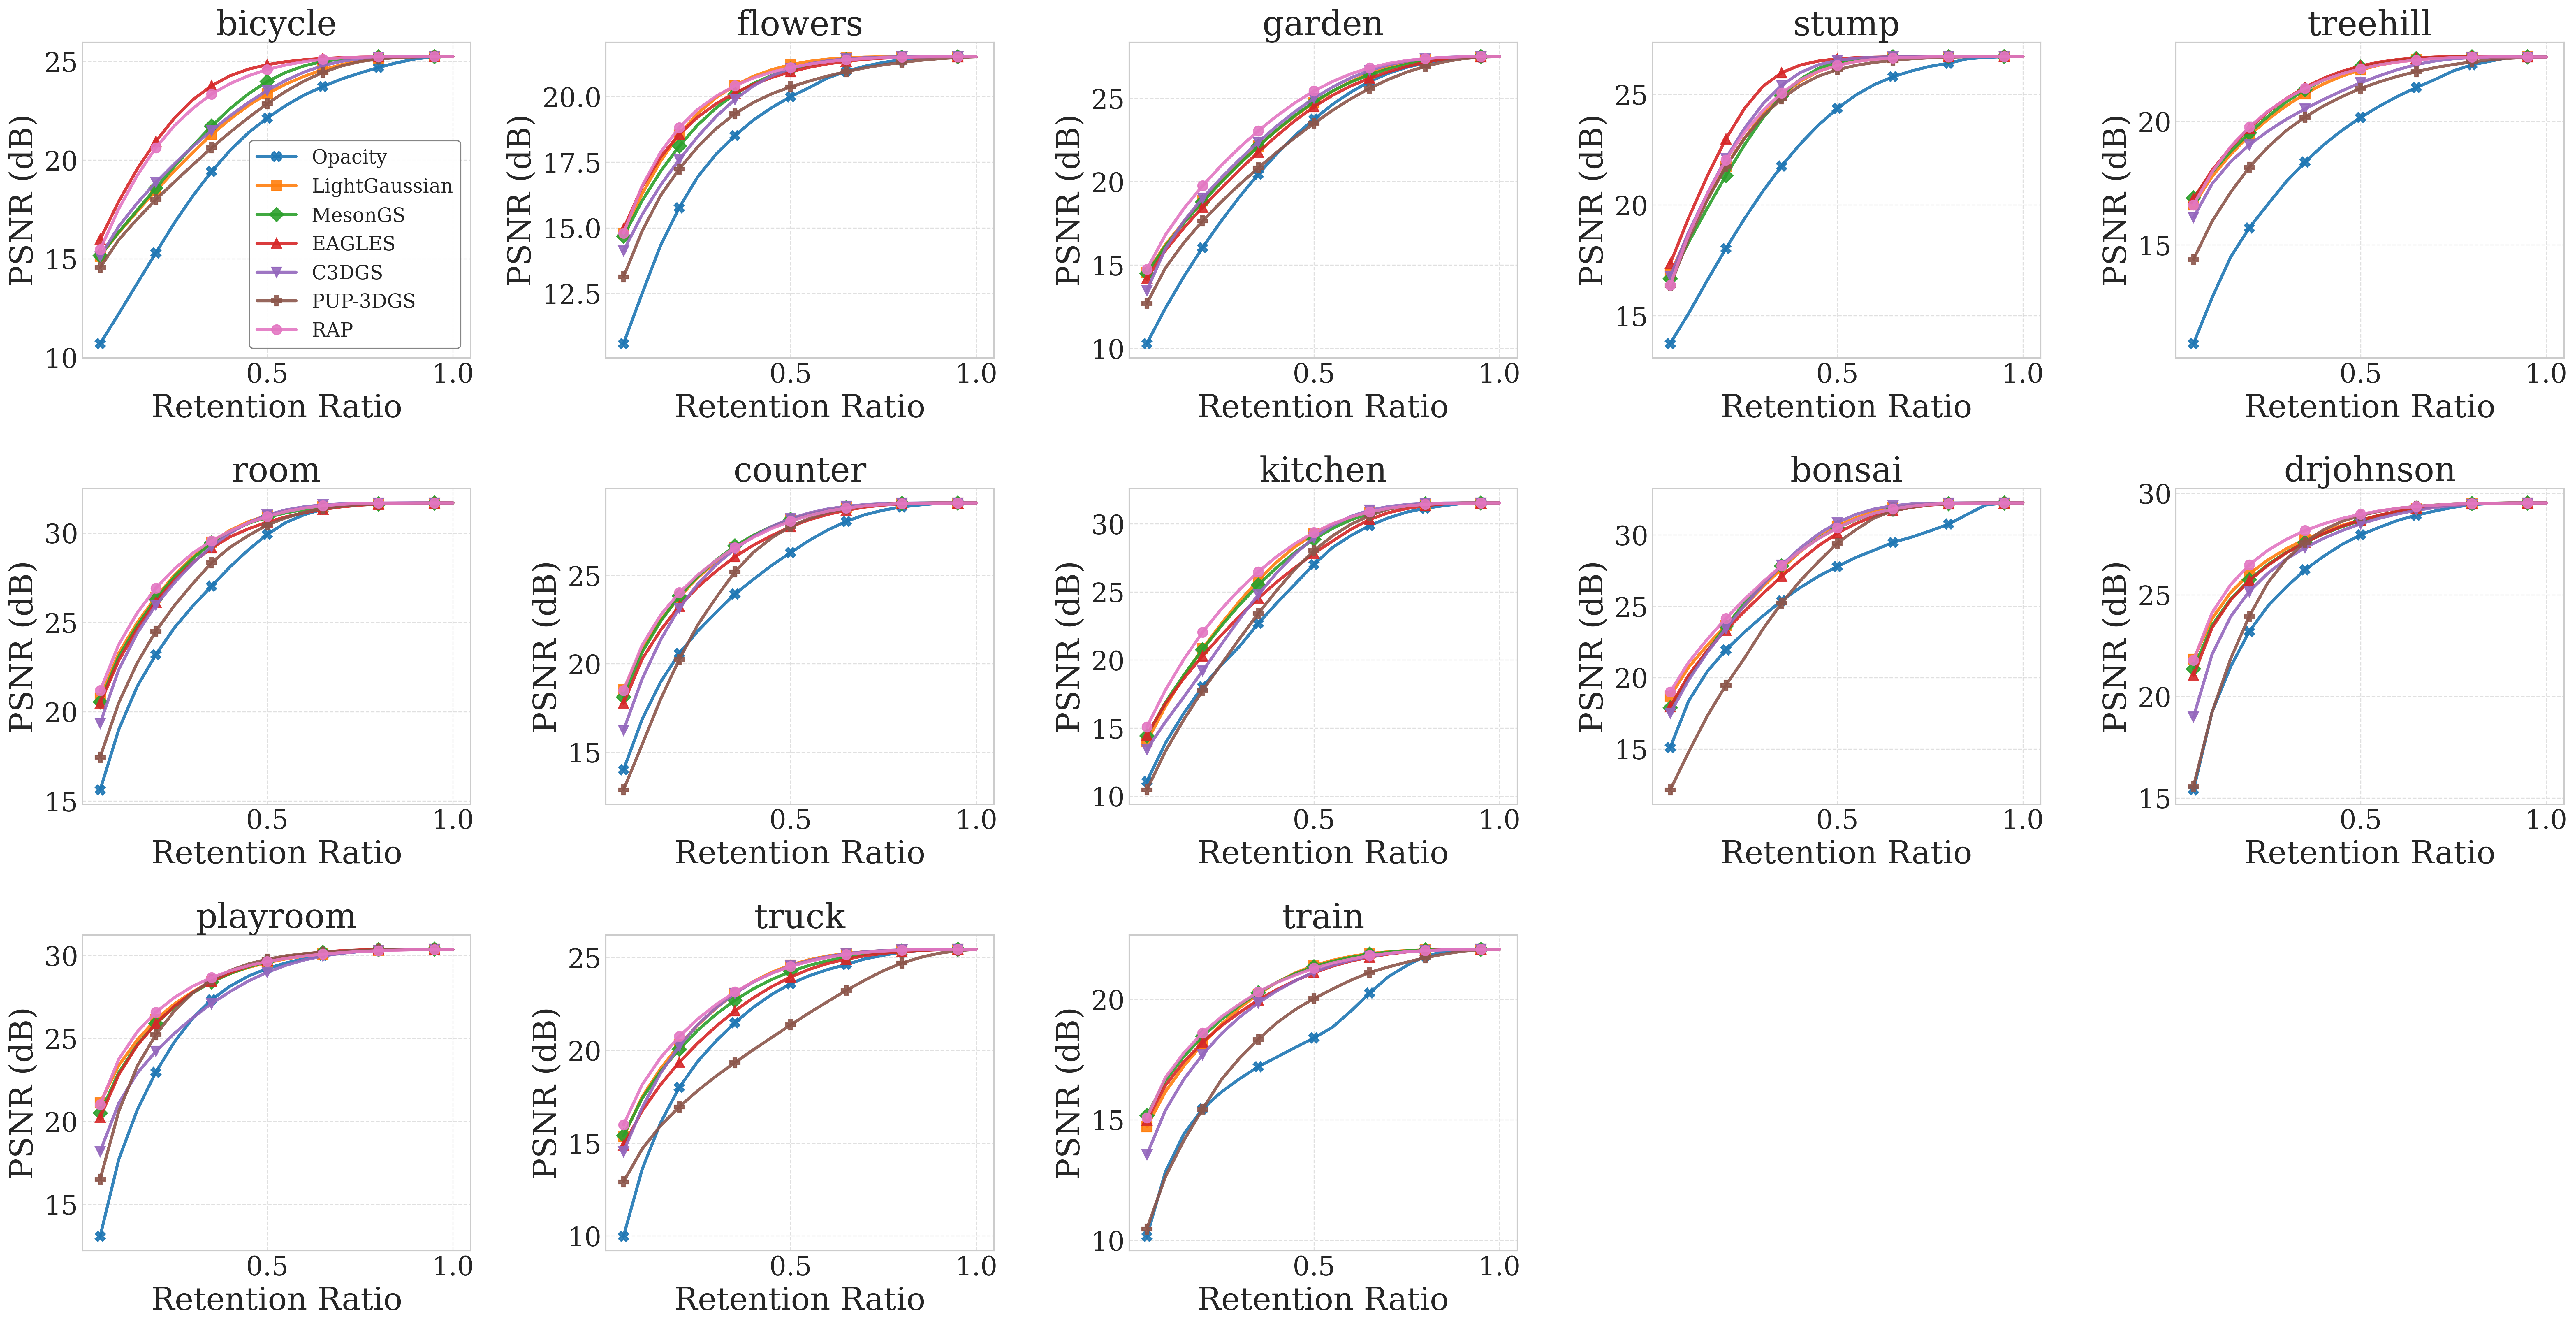
\includegraphics[width=\linewidth,height=0.31\textheight,keepaspectratio]{sec/imgs_sup/sup_2_psnr.png}
  \vspace{-3pt}
  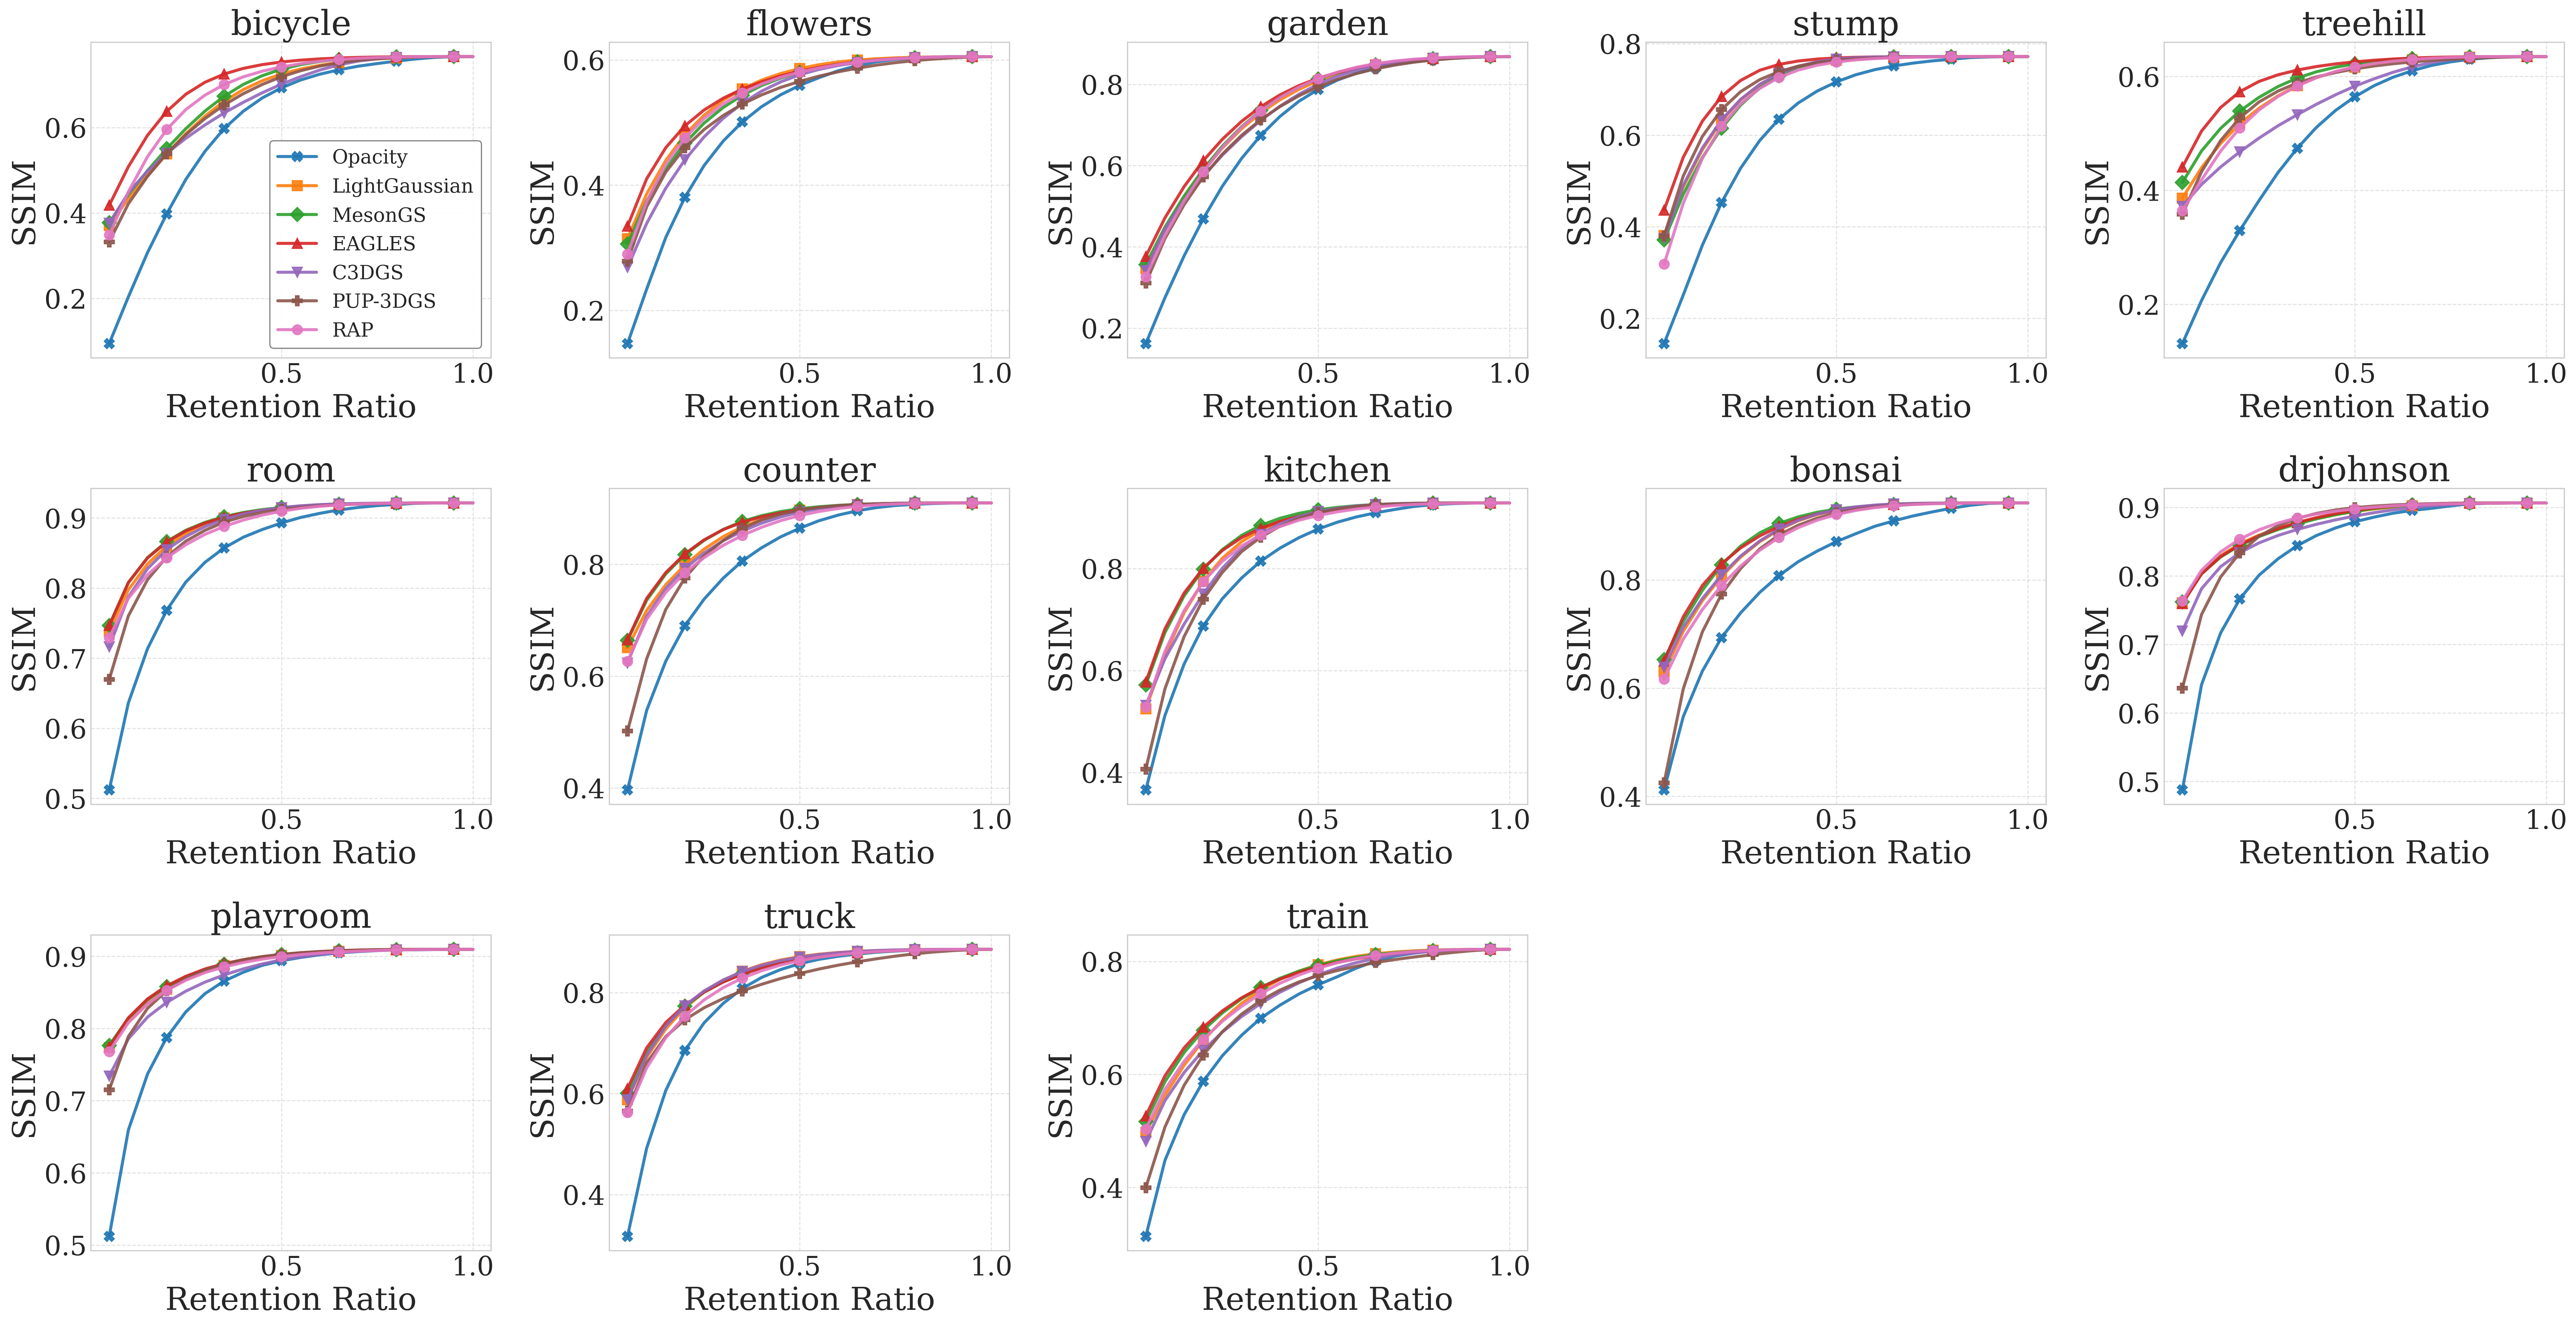
\includegraphics[width=\linewidth,height=0.31\textheight,keepaspectratio]{sec/imgs_sup/sup_2_ssim.png}
  \vspace{-3pt}
  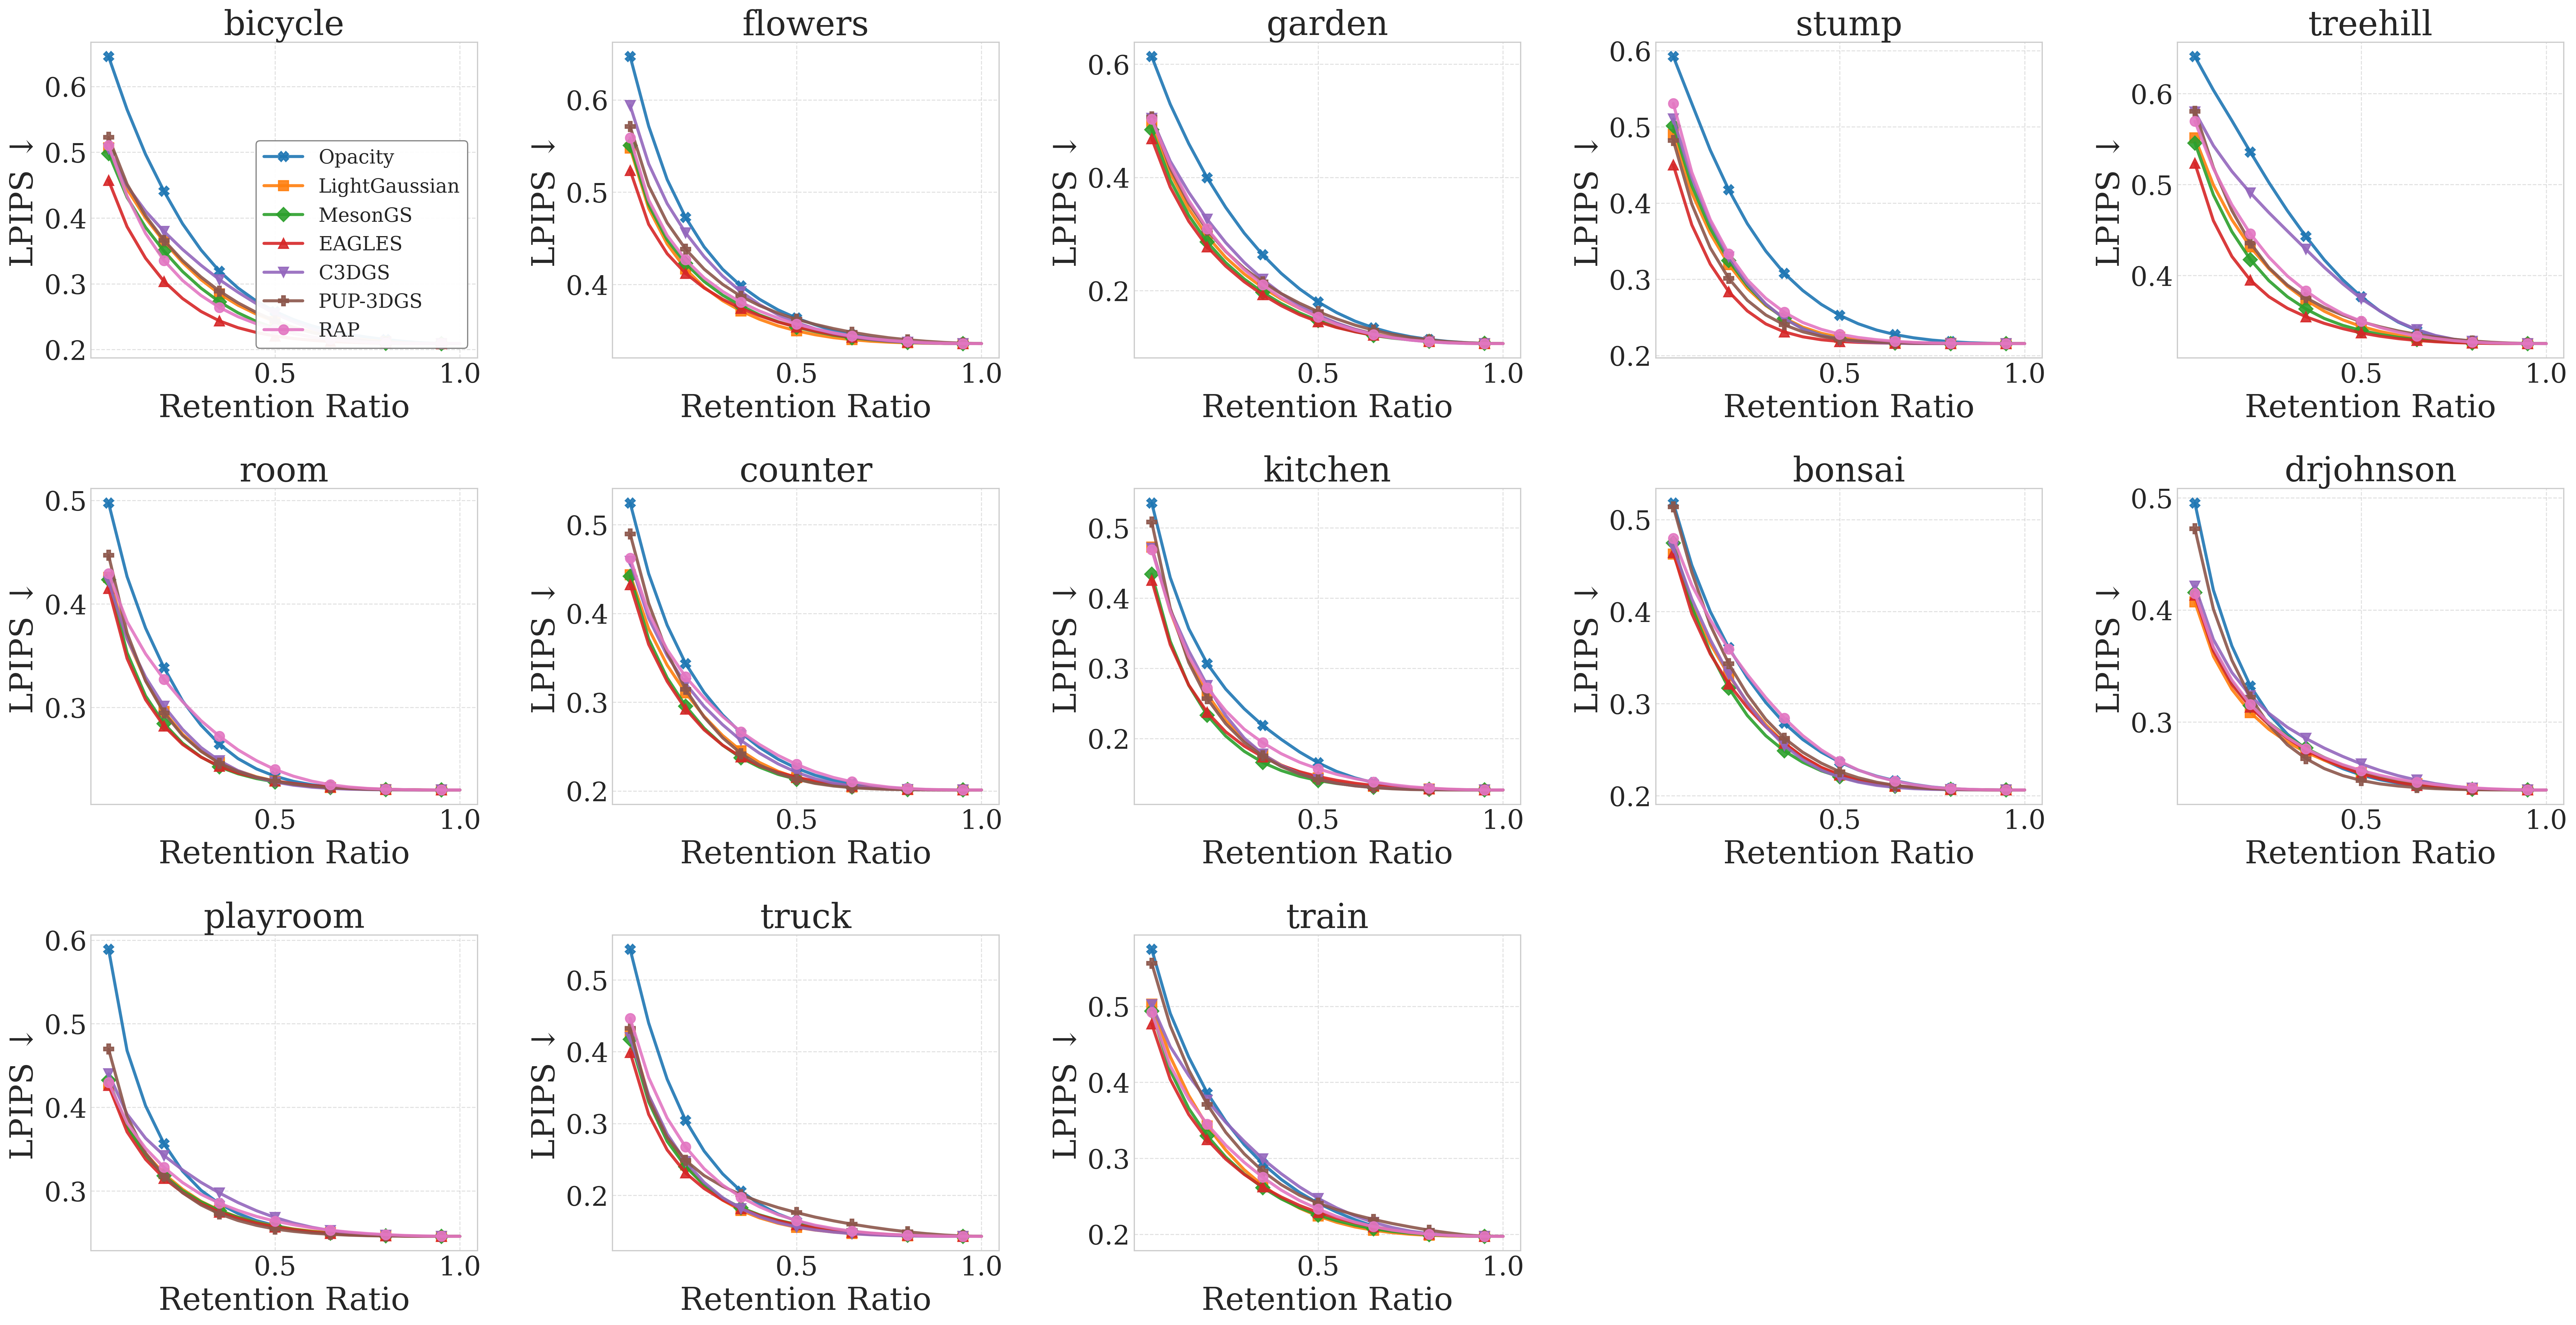
\includegraphics[width=\linewidth,height=0.31\textheight,keepaspectratio]{sec/imgs_sup/sup_2_lpips.png}
  \vspace{-6pt}
  \caption{
    Per-scene post-hoc pruning results across three metrics: 
    PSNR (top), SSIM (middle), and LPIPS (bottom).
  }
  \label{fig:sup_2_metrics}
\end{figure*}
